\documentclass[11pt]{article}
% --- Page and Typography ---
\usepackage[margin=1in]{geometry}
\usepackage{microtype}
\usepackage{parskip}
\usepackage{setspace}
\usepackage{enumitem}
\usepackage{titlesec}

\usepackage{amsmath,amssymb}
\usepackage{graphicx}
\usepackage{booktabs}
\usepackage{tikz}
\usepackage{fontawesome5}

\usepackage{amsthm}
\newtheorem{question}{Question}

% --- Font (modern look) ---
\usepackage{newpxtext,newpxmath}

% --- Colors and Links ---
\usepackage{xcolor}
\definecolor{aigold}{HTML}{9A6A18}
\definecolor{aigoldbg}{HTML}{FBF3DF}
\definecolor{aigoldln}{HTML}{E7D191}
\usepackage[colorlinks=true, linkcolor=blue!50!black, citecolor=purple!70!black, urlcolor=blue!70!black]{hyperref}

% --- AI-disclosure helpers -------------------------------------------------
% Banner placed at the top of every AI-drafted section.
\newcommand{\aibanner}{%
  \par\smallskip\noindent
  \setlength{\fboxsep}{7pt}%
  \fcolorbox{aigoldln}{aigoldbg}{%
    \parbox{\dimexpr\linewidth-2\fboxsep-2\fboxrule}{%
      \footnotesize\textcolor{aigold}{\faRobot~\textbf{AI-drafted section.}}%
      ~Synthesized from the cited literature; \textbf{pending author review}. Please verify claims and constants before relying on them.}}%
  \par\smallskip}

% --- Header/Footer ---
\usepackage{fancyhdr}
\pagestyle{fancy}
\fancyhf{}
\rhead{\thepage}
\lhead{Ali Vakilian}
\chead{\textit{An algorithmic perspective on fair clustering}}

% --- Section Styling ---
\titleformat{\section}{\large\bfseries\sffamily\color{blue!60!black}}{\thesection}{1em}{}
\titleformat{\subsection}{\normalsize\bfseries\sffamily\color{blue!40!black}}{\thesubsection}{1em}{}

\usepackage{natbib}

\title{Fair Clustering: Concepts, Methods, and Algorithms}
\author{Ali Vakilian \\ Department of Computer Science, Virginia Tech \\ {\sf vakilian@vt.edu}}
\date{Working draft -- June 2026}

\begin{document}
\maketitle

% ===== Abstract (AI-drafted) =====
\begin{abstract}
\noindent\textcolor{aigold}{\faRobot~\footnotesize\textbf{AI-drafted abstract.}}\\[2pt]
Clustering is a workhorse of unsupervised learning, yet classical objectives optimize only compactness and can entrench demographic disparities. This survey gives an algorithmic account of \emph{fair clustering}, organized around \emph{where} fairness is imposed. Part~I focuses on \textbf{group fairness}---balanced representation within clusters, demographic constraints on the chosen centers, and min-max (socially fair) cost---and reviews the approximation guarantees, hardness results, and core techniques (fairlet decomposition, LP rounding, coresets, tree embeddings, local search) that define the area. We also summarize individual fairness, proportionality and the core, and stability-based notions, and collect representative results (Table~\ref{tab:results}) and open problems.
\end{abstract}

% ===== Provenance & AI disclosure =====
\noindent\setlength{\fboxsep}{8pt}\fcolorbox{aigoldln}{aigoldbg}{\parbox{\dimexpr\linewidth-2\fboxsep-2\fboxrule}{%
\footnotesize\textcolor{aigold}{\faInfoCircle~\textbf{Provenance \& AI disclosure.}}\;
This document combines author-written material with clearly-marked AI-drafted sections.
\textbf{Author-written (Ali Vakilian):} Introduction, Group-Fairness Notions, Individual Fairness, Conclusion.
\textbf{AI-drafted (pending review):} Abstract, Preliminaries \& Notation (\S\ref{sec:prelim}), Proportionality/Core \& Stability (\S\ref{sec:prop}), Algorithmic Techniques (\S\ref{sec:tech}), Future Directions (\S\ref{sec:open}), and Table~\ref{tab:results}. AI-drafted sections also carry an inline banner.}}
\medskip

\section{Introduction}
Clustering is a foundational problem in machine learning and data analysis, aiming to partition a dataset into subsets (clusters) such that data points within a cluster are similar according to a given objective. Classical clustering algorithms, such as $k$-means, $k$-median, and $k$-center, have found widespread use in applications ranging from recommendation systems and market segmentation to medical diagnostics and image analysis. However, these traditional objectives focus solely on optimizing notions of proximity or compactness and often overlook issues of \emph{fairness}, particularly in how individuals from different demographic or social groups are treated.

In recent years, there has been a growing awareness that standard clustering procedures may exacerbate bias or reinforce structural disparities, such as forming clusters that disproportionately represent one demographic group while marginalizing others. This has motivated the development of \emph{fair clustering} algorithms, which aim to incorporate fairness constraints alongside standard clustering objectives. Fairness in clustering can take many forms, including ensuring balanced group representation within clusters, minimizing worst-case costs across demographic groups (social fairness), or guaranteeing that similar individuals are treated similarly (individual fairness). These models bring together algorithmic design with ethical and societal considerations, making the study of fair clustering both technically rich and socially important.

In this survey, we provide an overview of algorithmic results in fair clustering, with an emphasis on theoretical models, approximation guarantees, and algorithmic techniques. Our focus is primarily on \emph{centroid-based clustering} objectives, such as fair variants of $k$-center, $k$-median, and $k$-means, which have been the most extensively studied from an algorithmic perspective. We briefly mention other clustering frameworks where fairness has also been explored, including \emph{spectral clustering}~\citep{DBLP:conf/icml/KleindessnerSAM19,DBLP:conf/aistats/WangLDB23,tonin2025accelerating} and \emph{hierarchical clustering}~\citep{DBLP:conf/nips/AhmadianEK0MMPV20,DBLP:conf/afci/ChhabraSM21,DBLP:conf/icml/KnittelSDH23,DBLP:conf/nips/KnittelSDH23}, though these are not the main focus of this survey.

It is worth emphasizing that this is by no means a comprehensive survey. The body of work in fair clustering is vast and growing, including numerous models, fairness criteria, algorithmic strategies, and empirical evaluations. Our goal is to present a curated overview of core algorithmic contributions that have shaped the field, particularly in terms of theoretical guarantees and complexity results.
Moreover, we are not covering the empirical aspects of fair clustering in detail, such as the development of real-world benchmarks, practical deployment challenges, and critical evaluations of fairness definitions. These components are not only important but also essential for advancing the overall impact of fair clustering within the broader fields of algorithmic fairness and machine learning. Developing representative datasets and benchmarks is crucial for translating theoretical insights into effective practice, and deployment-focused studies often reveal practical trade-offs that are not captured by algorithmic models alone. For readers interested in these empirical and application-oriented directions, we point to the growing body of work that investigates the effectiveness of fair clustering on real datasets, examines benchmark design, and assesses the interplay between fairness, accuracy, and interpretability in real-world settings~\citep{chhabra2021overview,abbasi2021fair}. Well-known real-world examples, such as the ProPublica analysis of recidivism risk scores in classification~\citep{angwin2022machine}, have been instrumental in highlighting both the challenges and societal impact of fairness in algorithmic decision making. Similarly, compelling case studies and practical applications in fair clustering have the potential to capture attention and clearly demonstrate the real-world value and necessity of fairness in this area.

\paragraph{Roadmap of the survey.}
Fair clustering methods can be broadly categorized according to the type of fairness they seek to enforce, reflecting different philosophical and practical interpretations of what it means for a clustering to be \emph{``fair''}~\citep{dwork2012fairness,hardt2016equality,barocas2017fairness,mitchell2021algorithmic}. These categories distinguish whether fairness is defined at the level of individuals, groups, or the overall distribution of clustering outcomes, and each perspective introduces unique algorithmic challenges and modeling considerations.

% ===== AI-DRAFTED (pending author review) =====
% Auto-generated from survey/content.html by scripts/sync_html_to_tex.js — do not edit by hand.
\section{Preliminaries and Notation}\label{sec:prelim}
\aibanner

We collect the notation used throughout. An instance consists of a set of $n$ data points $P$ in a metric space $(X,d)$, where $d$ obeys the triangle inequality. A \emph{clustering} partitions $P$ into $k$ groups $\mathcal{C}=\{C_1,\dots,C_k\}$; in \emph{centroid-based} formulations each cluster $C_i$ is represented by a center $c_i$ from a candidate set $F\subseteq X$ (often $F=P$), and each point is assigned to its nearest open center.

\paragraph{Clustering objectives.} The three canonical objectives are unified by the $\ell_p$ cost of a center set $C$, $\mathrm{cost}_p(P,C)=\big(\sum_{x\in P} d(x,C)^p\big)^{1/p}$ with $d(x,C)=\min_{c\in C} d(x,c)$. Here $p=1$ is \textbf{$k$-median}, $p=2$ is \textbf{$k$-means} (sum of squared distances), and $p\to\infty$ is \textbf{$k$-center}, minimizing $\max_{x} d(x,C)$. All three are NP-hard, so the literature targets \emph{approximation} guarantees.

\paragraph{Protected groups.} Group fairness is defined relative to $\ell$ protected groups $P_1,\dots,P_\ell\subseteq P$ from a sensitive attribute. Groups may be \emph{disjoint} or \emph{overlapping}; $\Delta$ denotes the maximum number of groups any point belongs to ($\Delta=1$ when disjoint).

\paragraph{Approximation.} An $\alpha$-approximation returns a feasible (fair) solution of cost at most $\alpha$ times optimal. Many results are \emph{bicriteria}: an $(\alpha,\beta)$-approximation achieves cost within $\alpha$ of optimal while relaxing fairness by a slack $\beta$. Noting \emph{which} quantity is relaxed --- cost or fairness --- is essential when comparing results.

The taxonomy in Figure~1 organizes the notions surveyed below by \emph{where} fairness is enforced: within clusters, among centers, across group costs, or at the level of individuals and coalitions.

\section{Group Fairness Notions in Clustering}\label{sec:group-fairness}

A central line of work in fair clustering focuses on enforcing \emph{group fairness}, where individuals are partitioned into protected demographic groups (such as by race, gender, or age), and the goal is to ensure that the clustering process does not result in disproportionate or disparate treatment of any group. Group fairness has attracted significant interest due to its close connection to real-world equity concerns and its potential to reduce bias in downstream decision-making applications. The key idea is to ensure that no group is systematically underrepresented, overrepresented, or disproportionately burdened by the clustering output.

However, there is no single canonical definition of group fairness in clustering. Instead, several formalizations have been proposed, each capturing a different intuition about what it means for a clustering to be fair. These include notions such as \emph{balance within clusters}, where the demographic composition of each cluster should resemble that of the whole dataset; \emph{fair representation within centers}, where the selected cluster representatives (e.g., medoids or means) should be demographically diverse; and \emph{cost-based fairness} such as min-max or \emph{socially fair clustering}, which aims to equalize clustering costs across groups.

In the following subsections, we survey key algorithmic developments under each of these group fairness paradigms. 

% \begin{figure}[ht]
%     \centering
%     \begin{tikzpicture}[scale=1.2]
%       % Draw clusters
%       \draw[dashed, thick] (0,0) circle (1);
%       \draw[dashed, thick] (2.5,0.5) circle (1);
%       \draw[dashed, thick] (1.2,2) circle (1);

%       % Cluster centers
%       \fill[black] (0,0) circle (0.06);
%       \fill[black] (2.5,0.5) circle (0.06);
%       \fill[black] (1.2,2) circle (0.06);

%       % Points for cluster 1
%       \fill[red] (-0.4,0.3) circle (0.08);
%       \fill[blue] (0.5,0.4) circle (0.08);
%       \fill[red] (0.2,-0.6) circle (0.08);
%       \fill[blue] (-0.6,-0.4) circle (0.08);

%       % Points for cluster 2
%       \fill[blue] (2.8,0.2) circle (0.08);
%       \fill[red] (2.2,-0.2) circle (0.08);
%       \fill[red] (2.7,1.2) circle (0.08);
%       \fill[blue] (2,0.8) circle (0.08);

%       % Points for cluster 3
%       \fill[red] (0.9,1.3) circle (0.08);
%       \fill[blue] (1.5,2.3) circle (0.08);
%       \fill[red] (1.1,2.6) circle (0.08);
%       \fill[blue] (0.6,2.1) circle (0.08);

%       % Legend, moved to the right
%       \begin{scope}[shift={(4,1.5)}]
%         \fill[red] (0,1) circle (0.08); \node[right] at (0.2,1) {Group A};
%         \fill[blue] (0,0.7) circle (0.08); \node[right] at (0.2,0.7) {Group B};
%         \draw[dashed, thick] (0,0.4) circle (0.12); \node[right] at (0.2,0.4) {Cluster};
%       \end{scope}

%     \end{tikzpicture}
%     \caption{Illustration of fair clustering with two groups. Each cluster (dashed circle) contains a balanced mix of points from Group A (red) and Group B (blue).}
%     \label{fig:fair-clustering}
% \end{figure}

% \begin{figure}[ht]
% \centering
% \begin{tikzpicture}[scale=1.0, every node/.style={scale=1.0}]
%   % Coordinates for all points (same for both sides)
%   % Top row (Y=3.3 to 3.4)
%   \node[text=blue, scale=0.9]  (A) at (-4,3.4)    {\faFemale};  % in both clusters
%   \node[text=blue, scale=0.9]  (B) at (-3,3.4)    {\faFemale};  % in both clusters
%   \node[text=green!60!black, scale=0.9] (C) at (-2,3.4) {\faMale};     % in fair only
%   \node[text=green!60!black, scale=0.9] (D) at (-1,3.4) {\faMale};     % in fair only

%   % Second row
%   \node[text=blue, scale=0.9]  (E) at (-4.4,2.6)  {\faFemale};        % in unfair only
%   \node[text=green!60!black, scale=0.9] (F) at (-3.5,2.6) {\faMale};  % in both clusters
%   \node[text=blue, scale=0.9]  (G) at (-2.5,2.6)  {\faMale};
%   \node[text=green!60!black, scale=0.9] (H) at (-1.5,2.6) {\faFemale};

%   % Third row
%   \node[text=blue, scale=0.9]  (I) at (-4.2,1.8)  {\faMale};
%   \node[text=green!60!black, scale=0.9] (J) at (-3.2,1.8) {\faFemale};
%   \node[text=blue, scale=0.9]  (K) at (-2.2,1.8)  {\faMale};
%   \node[text=green!60!black, scale=0.9] (L) at (-1.2,1.8) {\faFemale};

%   % --- Left: Unfair cluster (3 blue females + 1 green male: A, B, E, F) ---
%   \draw[thick, blue!70!black] plot [smooth cycle, tension=1] coordinates {
%     (-4.2,3.5)    % A
%     (-2.8,3.6)    % B
%     (-3.5,2.7)    % F
%     (-4.6,2.7)    % E
%   };

%   % Dollar sign (left)
%   \node[text=yellow!80!black, scale=1.7] at (-3.7,3.0) {\$};

%   % Label (left)
%   \node at (-3,3.95) {\large\bfseries Unfair Clustering};

%   % --- Right: All points, mirrored ---
%   % Top row (Y=3.4)
%   \node[text=blue, scale=0.9]  at (2,3.4)   {\faFemale};   % in both clusters
%   \node[text=blue, scale=0.9]  at (3,3.4)   {\faFemale};   % in both clusters
%   \node[text=green!60!black, scale=0.9] at (4,3.4) {\faMale};      % in fair only
%   \node[text=green!60!black, scale=0.9] at (5,3.4) {\faMale};      % in fair only

%   % Second row
%   \node[text=blue, scale=0.9]  at (1.6,2.6)  {\faFemale};         % in unfair only
%   \node[text=green!60!black, scale=0.9] at (2.5,2.6) {\faMale};   % in both clusters
%   \node[text=blue, scale=0.9]  at (3.5,2.6)  {\faMale};
%   \node[text=green!60!black, scale=0.9] at (4.5,2.6) {\faFemale};

%   % Third row
%   \node[text=blue, scale=0.9]  at (1.8,1.8)  {\faMale};
%   \node[text=green!60!black, scale=0.9] at (2.8,1.8) {\faFemale};
%   \node[text=blue, scale=0.9]  at (3.8,1.8)  {\faMale};
%   \node[text=green!60!black, scale=0.9] at (4.8,1.8) {\faFemale};

%   % --- Right: Fair cluster (2 blue females + 2 green males: A, B, C, D mirrored) ---
%   \draw[thick, blue!70!black] plot [smooth cycle, tension=1] coordinates {
%     (1.8,3.5)    % A
%     (3.2,3.6)    % B
%     (4.8,3.5)    % D
%     (3.7,2.7)    % C (was F in left, but use top left 2 blue, top left 2 green)
%   };

%   % Dollar sign (right)
%   \node[text=yellow!80!black, scale=1.7] at (3.4,3.0) {\$};

%   % Label (right)
%   \node at (3.5,3.95) {\large\bfseries Fair Clustering};

%   % -- Legend (right) --
%   \begin{scope}[shift={(6,2.8)}]
%     \node[text=blue, scale=0.9] (L1) at (0,0.8) {\faFemale};
%     \node[right] at (0.3,0.8) {Group 1};
%     \node[text=green!60!black, scale=0.9] (L2) at (0,0.4) {\faMale};
%     \node[right] at (0.3,0.4) {Group 2};
%     \node[text=yellow!80!black, scale=0.9] at (0,0) {\$};
%     \node[right] at (0.3,0) {Resource};
%   \end{scope}
% \end{tikzpicture}
% \caption{
% \textbf{Left:} Unfair clustering, with a cluster containing 3 blue females and 1 green male.
% \textbf{Right:} Fair clustering, with a cluster containing 2 blue females and 2 green males. The same set of individuals are clustered differently to illustrate the effect of fairness constraints. Icons indicate individuals from two groups (e.g., by gender or demographic feature).
% }
% \label{fig:fair-unfair-clustering-same-layout}
% \end{figure}


\begin{figure}[ht]
    \centering
    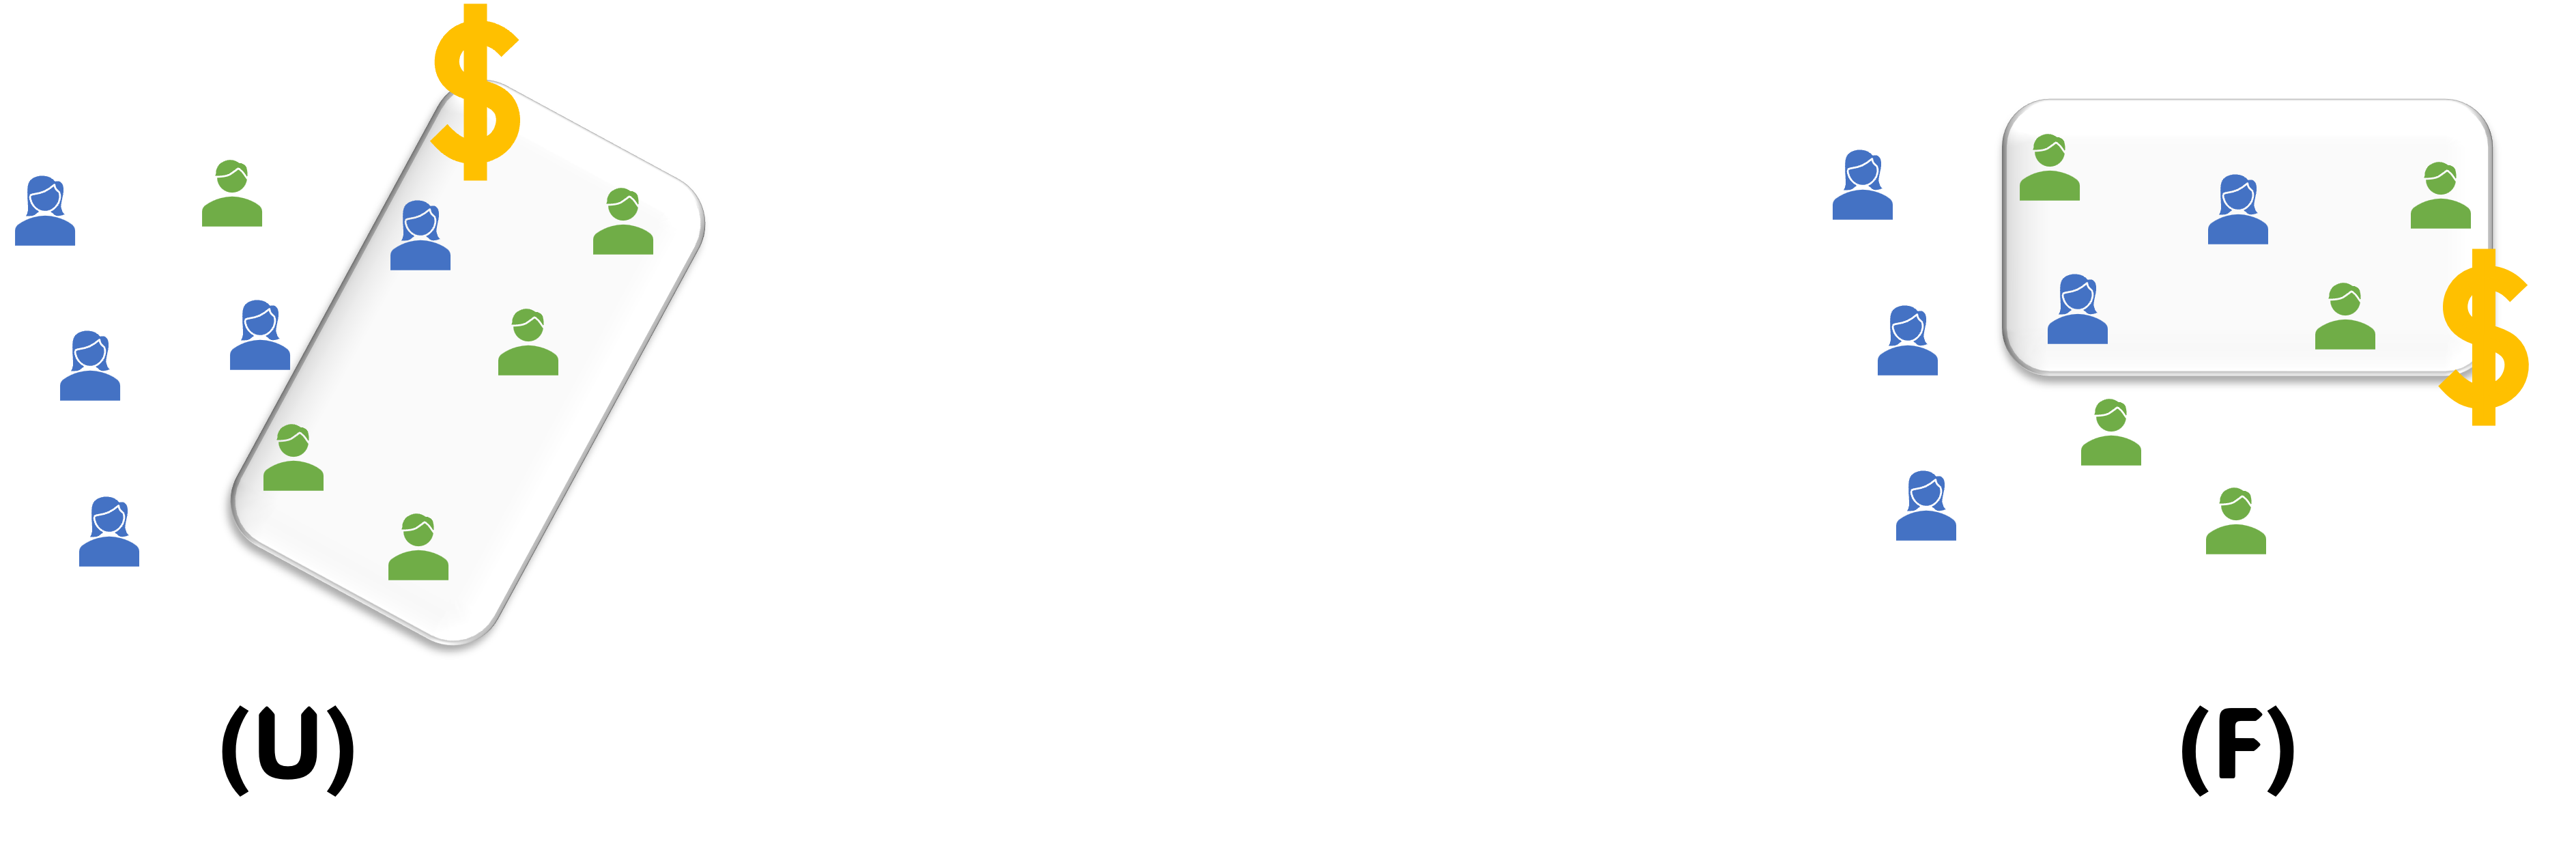
\includegraphics[width=0.75\textwidth]{images/bal_rep_cluster.png}
    \caption{
        \textbf{Left $(\mathsf{U})$:} An unbalanced clustering, where the selected cluster is dominated by individuals from one group (green), with only a single member from the other group, resulting in unequal representation in the advantaged cluster. \textbf{Right (F):} A more balanced clustering.
    }
    \label{fig:bal_rep_clustering}
\end{figure}


\subsection{Fair representation within clusters}
This notion of group fairness in clustering aims to ensure that each cluster reflects the demographic composition of the dataset, particularly across protected groups such as gender or ethnicity. \citet{DBLP:conf/nips/Chierichetti0LV17} pioneered the algorithmic study of fair clustering by introducing the notion of \emph{balance}, a quantitative measure of group parity within a subset.





In their seminal work, \citet{DBLP:conf/nips/Chierichetti0LV17} introduced the notion of fair clustering with two protected groups. In this setting, we are given a set of $n$ points $P$ in a metric space $(X, d)$, where each point belongs to either the \emph{red} or the \emph{blue} group. For any subset of points $S \subseteq P$, let $r(S)$ and $b(S)$ denote the number of red and blue points in $S$, respectively. The balance is defined as $\text{balance}(S) = \min\left( \frac{r(S)}{b(S)}, \frac{b(S)}{r(S)} \right)$, which attains its maximum value of $1$ when the groups are equally represented. Given the point set $P$, a number of clusters $k$, and a required minimum balance $t \in (0,1]$, the fair clustering problem is to partition $P$ into clusters $\mathcal{C} = \{C_1, \dots, C_k\}$ such that each cluster $C_i$ satisfies $\text{balance}(C_i) \geq t$, a property referred to as $t$-balance, while minimizing a clustering objective such as $k$-center or $k$-median.

\cite{DBLP:conf/nips/Chierichetti0LV17} showed that enforcing exact fairness constraints in clustering is {\bf NP}-hard, and then developed a two-stage approximation framework based on the concept of \emph{fairlets} which are small, $t$-balanced subsets that act as ``atomic'' units in the subsequent clustering process. 
The method first decomposes the dataset into a collection of fairlets and then applies standard clustering algorithms on their representatives. For the case of $t = 1$, the fairlet decomposition reduces to a minimum-cost perfect matching problem. Their framework yields approximation algorithms when the balance parameter $t$ is a rational number: For example, they provide a $4$-approximation for the fair $k$-center problem, and show $O(t)$-approximation for the fair $k$-median problem.

This two-step method preserves fairness guarantees and modularity which allows existing clustering algorithms to be adapted with minimal changes. However, the construction of fairlets may become computationally expensive, particularly as the number of groups increases. 

Next, we consider a generalization of the fair clustering problem to the setting with multiple groups. Specifically, we are given a set of $n$ points $P$ in a metric space $(X, d)$, where each point may belong to one or more of $\ell$ (possibly overlapping) groups $P_1, \dots, P_\ell$, and $P = \bigcup_{i \in [\ell]} P_i$.

\subsubsection{Extending to multiple groups: (I) absolute balance.} 
Generalizing the fair representation notion of \citet{DBLP:conf/nips/Chierichetti0LV17}, \citet{bera2019fair} introduced a more general model of fairness in clustering using parameterized group constraints applicable to the setting with more than two groups. Each protected group $j$ is assigned lower and upper fraction bounds, $\alpha_j$ and $\beta_j$, to enforce representation constraints in every cluster. Formally, a clustering $\mathcal{C} = \{C_1, \cdots, C_k\}$ is {\em $(\alpha, \beta)$-fair} if for every cluster $C\in \mathcal{C}$ and every group $j\in [\ell]$, $\alpha_j \cdot |C| \le |C \cap P_j| \le \beta_j \cdot |C|$. 


\citet{bera2019fair} present a \emph{post-processing algorithm} that converts any vanilla clustering (for any $\ell_p$ objective, such as $k$-means, $k$-median, or $k$-center) into one that satisfies these fairness constraints, with an additive violation of at most $4\Delta + 3$ individuals per group per cluster (where $\Delta$ is the maximum number of groups any point belongs to), while increasing the clustering cost by at most a constant factor. Independently,~\citet{DBLP:conf/approx/Bercea0KKRS019} obtained similar guarantees by allowing small additive violations in group representation. While both approaches seek to balance fairness and clustering quality, the algorithm of~\citet{bera2019fair} provides stronger guarantees and supports the more general setting with overlapping group memberships.

For fair $k$-center clustering, \citet{DBLP:conf/nips/HarbL20} proposed a scalable algorithm that achieves a 5-approximation guarantee, with additive fairness violations matching those in \citet{bera2019fair}. Notably, although this algorithm allows for worst-case additive violations of fairness constraints, the authors show that the expected additive deviation from the specified $\alpha_i$ and $\beta_i$ bounds is zero\footnote{That is, the group representation bounds are satisfied on average, as opposed to expected zero violations.}. 

By designing coresets for fair clustering,~\citet{DBLP:conf/icalp/BandyapadhyayFS21} presented algorithms that compute a constant-factor approximation for fair $k$-median and $k$-means, running in time $(k\Delta)^{O(k\Delta)} \mathrm{poly}(n)$, and crucially, these algorithms do not violate the fairness constraints. In the special case of no overlap between groups, the runtime improves to $(k\ell)^{O(k\ell)} \mathrm{poly}(n)$. Previously, coresets for fair representation clustering were also studied in~\citep{DBLP:conf/waoa/0001SS19,DBLP:conf/nips/HuangJV19}.

Prior to~\citep{bera2019fair}, this notion of fairness was studied for (1) the $k$-center problem~\citep{rosner2018privacy}, and (2) $k$-clustering with an $\ell_p$-objective on balanced instances, which are instances with equal group sizes and $\alpha_j = \beta_j = 1$ for all $j \in [\ell]$~\citep{DBLP:journals/orl/BohmFLMS21}. In these special cases, the fair clustering problem admits a constant-factor approximation.
In another line of research, a special case of this fairness notion, known as \emph{restricted dominance}, imposes only upper bounds on the fraction of each group within clusters. For this setting, \citet{ahmadian2019clustering} developed a bicriteria approximation algorithm that provides fairness guarantees with bounded additive violations 

Building on~\citep{bera2019fair,backurs2019scalable}, \citet{DBLP:conf/fat/DaiMV22} designed a ``purely multiplicative'' $O(\log k)$-approximation for the $k$-median objective (i.e., without additive violations) in the setting with multiple groups, under the $(\alpha, \beta)$ fairness notion of~\citep{bera2019fair}. Their algorithm runs in time $n^{O(\ell)}$, where $\ell$ is the number of groups. It was subsequently shown by~\citet{bandyapadhyay2024polynomial} that obtaining an approximation factor of $o(\log k)$ for fair $k$-median in \emph{polynomial time} is as hard as breaking the long-standing $\Omega(\log k)$ barrier for the well-studied \emph{soft uniform capacitated $k$-median} problem. The approach of~\citet{DBLP:conf/fat/DaiMV22} relies on probabilistically approximating arbitrary metrics by tree metrics~\citep{bartal1998approximating,fakcharoenphol2003tight}. Notably, in the context of fair $k$-median, this idea of approximating the input metric with a distribution over dominating trees was also used by~\citet{backurs2019scalable} in their \emph{near-linear time} approximation algorithm for fair representation clustering with two groups.


%\textcolor{red}{Check the intro of the paper. There are some missing prior work. In particular coreset construction}

\begin{question}\label{q:approx-log}
Can the $O(\log k)$-approximation barrier for fair $k$-median under multi-group $(\alpha, \beta)$ fairness constraints be improved in polynomial time, or is this limitation fundamental?
\end{question}
\begin{question}\label{q:near-linear-time}
Is it possible to design a near-linear time approximation algorithm for fair $k$-clustering with general $\ell_p$ objectives under multi-group $(\alpha, \beta)$ fairness constraints? In particular, can we obtain algorithms that are both efficient and provide strong approximation guarantees for settings beyond two groups and objectives beyond $k$-median?
\end{question}
\subsubsection{Extending to multiple groups: (II) pairwise}
In a different extension of the fair representation within clusters to multiple groups,~\cite{bandyapadhyay2024polynomial,bandyapadhyay2025constant} explicitly studied the notion of {\em pairwise} fairness which given an integer parameter $t$, requires to output a clustering $\mathcal{C}=\{C_1,\cdots,C_k\}$ such that for every cluster $C\in \mathcal{C}$, and every pair of groups $i,j\in [\ell]$, $|C\cap P_i| /t\le |C\cap P_j| \le t\cdot |C\cap P_i|$.

For $k$-center, via an LP-based rounding scheme,~\citet{bandyapadhyay2025constant} show an $O(1)$-approximation for two settings: (i) there are two groups in the input and $t$ is an integer, and (ii) when $t=1$. On the hardness side, the authors prove an integrality gap of $\Omega(k)$ for their proposed LP relaxation when $t$ is not an integer even with two groups. 

For $k$-median, the problem turns out to be more difficult. \citet{bandyapadhyay2024polynomial} provide an $O(k^2 \ell t)$-approximation for $t$-pairwise fair $k$-clustering when there are $\ell$ disjoint groups in the input. On the negative side, they show it is NP-hard to approximate the problem within a factor better than $n^{1-\varepsilon}$, for every constant $\varepsilon>0$, when there are {\em overlapping groups}, even for $k=2$.



\subsubsection{Further remarks}
\paragraph{Fair clustering with Sum-of-Radii objective.} This notion has been popular and well-studied for clustering with other objective function such as sum-of-radii, where the goal is to minimize the sum of radii of the constructed clusters~\citep{carta2024fpt,nezhad2025polynomial}. 
    
\paragraph{Fairness under bounded cost.}
Another research direction focuses on minimizing unfairness given an upper bound on the clustering cost, as proposed by~\citet{DBLP:conf/nips/EsmaeiliBSD21}. Instead of minimizing clustering cost subject to strict fairness constraints, this approach sets an upper limit on the clustering cost and shifts the objective to minimizing unfairness. In this setting, each point belongs to a group, and clusters are required to approximately reflect the population proportions of each group. Formally, unfairness for group $j$ is defined as the minimum proportional relaxation $\delta_j$ such that, in every cluster, the group's proportion lies within the relaxed bounds $[\alpha_j - \delta_j, \beta_j + \delta_j]$. The paper considers three natural objectives: \emph{group-utilitarian} (minimize the sum of all group violations), \emph{group-egalitarian} (minimize the maximum group violation), and \emph{group-leximin} (minimize the worst, then the second-worst, and so on, violations). The optimization problem can be formally stated as minimizing one of these \emph{unfairness objectives}, subject to the constraint that the clustering cost does not exceed a given threshold $U$. For the first two fairness objectives, the authors provide bicriteria approximation algorithms that achieve bounded violations of the fairness constraints, and ensure that the objective value is within a small additive error of the upper bound $U$. 

\paragraph{Fair labeled clustering.} Clustering is a widely used preprocessing step in many decision-making pipelines. From a fairness perspective, it is often sufficient to ensure equity in the outcomes or labels assigned to clusters in subsequent steps, rather than enforcing group balance within the clusters themselves. Motivated by these applications, \citet{esmaeili2022fair} introduced the fair labeled clustering framework, where fair representation constraints are imposed on the set of points that receive each outcome label. Specifically, after clusters are formed, the goal is to ensure that, for each label, the aggregate population assigned that label satisfies the desired group representation, even if individual clusters do not. This approach is less restrictive than traditional fair clustering and often results in higher-quality clusterings, while still mitigating disparate impact in the outcomes.

The fair labeled clustering problem has two main variants. In the first, \emph{labeled clustering with assigned labels (LCAL)}, each cluster is given a predetermined outcome label (for example, based on the cluster center). In the second, \emph{labeled clustering with unassigned labels (LCUL)}, labels can be assigned to clusters in a way that further improves fairness or efficiency. In both cases, the goal is to minimize clustering cost while satisfying proportional group representation constraints for each label. Notably, LCAL can be solved in polynomial time for any fixed number of labels, in contrast to the traditional fair clustering problem, which is {\bf NP}-hard (even not known whether it is possible to approximate within a factor better than $\Omega(\log k)$). The authors develop efficient algorithms based on network flow for both settings, as well as randomized rounding for LCUL to ensure fairness constraints hold in expectation.

    %The fair labeled clustering problem comes in two main variants: (1) \emph{Labeled Clustering with Assigned Labels (LCAL)}, where the outcome assigned to each cluster is fixed (for instance, based on the cluster center), and (2) \emph{Labeled Clustering with Unassigned Labels (LCUL)}, where labels can be assigned to clusters in a way that further improves fairness or efficiency. For both settings, the objective is to minimize the clustering cost subject to proportionality constraints on the group representation within each label (possibly with additional size or budget constraints per label). Notably, the LCAL problem can be solved in polynomial time for any fixed number of labels, a sharp contrast to the traditional fair clustering problem, which is {\bf NP}-hard. %Efficient algorithms and network-flow based methods are provided for both variants, with further randomized rounding techniques for the more general LCUL case, ensuring fairness constraints are satisfied in expectation.

\paragraph{Distance to fairness and consensus.} \citet{chakraborty2025towards} introduced the problem of finding the closest fair clustering to a given clustering in the case of binary groups, and devised a constant-factor approximation algorithm for it. They also proposed the notion of fair consensus clustering, where, given a collection of clusterings $\mathcal{D}_1, \ldots, \mathcal{D}_m$ over the same dataset, the goal is to find a fair clustering $\mathcal{C}^*$ that minimizes the overall distance to the input clusterings. The distance is defined as the $\ell_p$-norm of the vector of distances from $\mathcal{C}^*$ to each $\mathcal{D}_i$, where the distance between two clusterings is the number of pairs of points that are clustered together in one clustering but not in the other. For this consensus problem, they show that their approach for closest fair clustering yields a constant-factor approximation in the two-group setting.  

\begin{question}
    Is it possible to generalize the results of~\cite{chakraborty2025towards} for closest fair clustering and fair consensus clustering to settings with more than two groups?
\end{question}

\paragraph{In large-scale computational models.}
In the context of fair clustering, with fair representation within clusters, under massive data processing models, streaming algorithms have received increasing attention due to the need to process large-scale and rapidly arriving data. A key challenge in this setting is to ensure fairness, typically defined via demographic constraints or group-based balance, while maintaining computational and memory efficiency. In the standard insertion-only streaming model, several works have explored the use of \emph{coresets} for fair $k$-means and $k$-median clustering~\citep{DBLP:conf/waoa/0001SS19,DBLP:conf/nips/HuangJV19,DBLP:conf/icalp/BandyapadhyayFS21}, providing algorithms that maintain compact summaries (coresets) of the input while approximately preserving both clustering cost and fairness constraints. These approaches allow for efficient post-processing to recover fair clusterings and have established bounds on coreset sizes and approximation guarantees. However, adapting fairness to more dynamic models like the \emph{sliding window model}, where only the most recent elements are considered, remains more challenging. The recent work of~\citet{cohenfair25} initiates the study of fair clustering in this setting, providing the first algorithms for fair $k$-center clustering in sliding windows with provable approximation and space guarantees. 
%Despite this progress, several open questions remain, such as developing streaming algorithms for fair $k$-means or $k$-median clustering in sliding windows, improving coreset sizes under fairness constraints, and handling more complex or intersectional group fairness definitions in real-time. Bridging the algorithmic techniques between insertion-only, sliding window, and turnstile models under fairness constraints is a promising and largely unexplored direction.


%\textcolor{red}{sliding windows streaming~\cite{cohenfair25}. streaming and coreset~\cite{DBLP:conf/waoa/0001SS19,DBLP:conf/nips/HuangJV19,DBLP:conf/icalp/BandyapadhyayFS21}}



\subsubsection{Fair representation within centers (Centroid-based clustering)}
Another important fairness notion in clustering is \emph{fair representation among centers}, where the demographic composition of the selected cluster centers themselves must reflect a desired distribution. This idea is particularly relevant in centroid-based clustering objectives such as $k$-center, $k$-median, and $k$-means, especially when the centers are intended to serve as a representative summary of the dataset (e.g., in applications like data summarization or decision-making).

\citet{kleindessner2019fair} introduced a formulation where the dataset is partitioned into $\ell$ demographic groups, and exactly $k_i$ centers must be chosen from group $i$, for some input parameters $k_1, \dots, k_\ell$. While this ensures strict demographic proportionality, it may significantly degrade clustering quality. To address this,~\citep{hotegni2023approximation,nguyen2022fair} proposed a relaxation called \emph{fair range clustering}, which requires the number of selected centers from each group $i$ to fall within a specified interval $[\alpha_i, \beta_i]$. This flexible model captures a range of fairness policies while allowing for improved clustering performance. They present constant-factor approximation algorithms for fair range $k$-clustering under $\ell_p$-norm objectives, including $k$-center, $k$-median, and $k$-means.

%Earlier works like those by Kleindessner et al.~\cite{kleindessner2019fair} and its follow-up~\cite{awasthi2020fair} also investigate fairness in data summarization via center-constrained formulations, providing approximation algorithms under fairness constraints. Notably, approximation guarantees are often traded for fairness: for example, \cite{kleindessner2019fair} provides a 5-approximation algorithm for the strict fairness-constrained $k$-center problem.

Overall, fair representation within centers is crucial in applications like image search, recourse design, or any setting where the selected representatives are presented directly to users or downstream decision-making systems.

%\paragraph{Clustering under matroid constraints.}
\paragraph{Further remarks.} 
Clustering with constraints on the \emph{set of centers} that form an independent set of a matroid over the candidate facilities is a well-studied abstraction that subsumes this notion of fairness. This line of work has yielded constant-factor approximations through LP relaxations with matroid polytopes, swap/pipage rounding, and matroid-aware local search, across median/means/center-style objectives, and has been used extensively in the fair-clustering literature~\citep{hajiaghayi2010budgeted,krishnaswamy2011matroid,charikar2012dependent,swamy2016improved,chen2016matroid,krishnaswamy2018constant,jones2020fair,chiplunkar2020solve}. 
In particular, the notion of fairness with exact per-group quotas is a direct special case (a partition-matroid feasibility on centers), placing it squarely within this framework; by contrast, the \emph{fair range} variant relaxes quotas to intervals and is not itself a matroid (since feasibility is not downward-closed), though it admits reductions that leverage matroid structure via extendable-set relaxations in~\citep{el2020fairness, hotegni2023approximation}. 
%Despite this close connection, and although matroid-constrained clustering \emph{per se} is well studied in fair clustering, this natural generalization---imposing center-side fairness directly (and, in the range case, interval constraints) across $\ell_p$-objectives with the guarantees we target here---has not been systematically addressed in prior fair-clustering work.

\subsubsection{Min-Max fairness (aka socially fair clustering)}

Socially fair clustering addresses disparities in clustering cost across different demographic groups. Rather than requiring fair representation within each cluster, the objective here is to minimize the worst-case (maximum) clustering cost incurred by any group. Early work by \citet{abbasi2021fair} and \citet{ghadiri2021socially} introduced this formulation for $k$-median and $k$-means objectives, providing $O(\ell)$-approximation algorithms, where $\ell$ is the number of protected groups. However, their results relied on natural LP relaxations that were shown to have an integrality gap of $\Omega(\ell)$, limiting the scope for improved approximations.

To address this limitation, \citep{makarychev2021approximation} introduced a strengthened LP relaxation for socially fair $\ell_p$-clustering that adds locality constraints tailored to the structure of the metric space and the weight distribution. Their algorithm achieves an $\tilde{O}(\log \ell / \log \log \ell)$-approximation for general $p$, which is tight under standard complexity assumptions—matching a hardness lower bound for even unweighted $k$-median on uniform metrics~\cite{bhattacharya2014new}. This result represents the best-known approximation for socially fair $k$-median and $k$-means (for $p = 1$ and $p = 2$), and generalizes to arbitrary weights over groups. Moreover, \citep{makarychev2021approximation} extend their techniques to the weighted case, where each group $j$ is represented by a weight function $w_j : L \rightarrow \mathbb{R}_+$ over the set of data points, and the goal is to minimize $\max_j \sum_{v \in L} w_j(v) \cdot d(v, C)^p$ for a center set $C$. This framework captures applications where group importance varies across the domain, and it broadens applicability to non-disjoint and even overlapping group memberships.

Finally, their algorithm supports both multiplicative and bicriteria approximation guarantees. The bicriteria version relaxes the number of centers from $k$ to $k/(1-\gamma)$ and achieves a cost approximation of $O(1/\gamma)$ times the optimum. Overall, this line of work solidifies min-max fairness as a practically and theoretically robust approach to equitable clustering across heterogeneous populations.

\cite{DBLP:conf/soda/ChlamtacMV22} extended the socially fair clustering framework to a more general family of objectives called $(p, q)$-fair clustering, where the goal is to minimize the $\ell_q$ norm across groups of the $\ell_p$ clustering cost incurred by each group. This formulation captures and generalizes a wide range of clustering problems: classical clustering ($q = p$), robust clustering ($q = 1$)~\cite{anthony2010plant}, and socially fair clustering ($q = \infty$). The $(p, q)$ objective provides a flexible way to interpolate between average-case fairness and worst-case fairness, allowing practitioners to tune the fairness strictness by adjusting $q$ relative to $p$.

The authors developed approximation algorithms based on novel convex programming relaxations. For the case $p \leq q$, they achieved an $O((q / \ln(1 + q/p))^{1/p})$-approximation using randomized rounding and careful handling of integrality gaps through non-standard constraints. For the case $p \geq q$, they presented an $O(k^{(p-q)/(2pq)})$-approximation, which nearly matches their derived hardness bound of $k^{\Omega((p-q)/(pq))}$ under standard assumptions, such as the hardness of the Min-$s$-Union problem. These results nearly close the gap between algorithmic upper bounds and known lower bounds for various $p$, $q$ regimes. Overall, the $(p, q)$-fair clustering model provides a powerful framework for balancing fairness and efficiency in clustering, accommodating a range of practical fairness requirements beyond strict max-min fairness.

\cite{DBLP:journals/ipl/GoyalJ23} provided \emph{tight fixed-parameter tractable (FPT)} $(3^z + \varepsilon)$-approximation algorithms for socially fair $k$-median ($z=1$) and $k$-means ($z=2$), running in time $(k/\varepsilon)^{O(k)} \cdot n^{O(1)}$, and proved these bounds to be optimal under the \emph{Gap-ETH} assumption.


The min-max fairness framework has since been influential in formalizing fairness in clustering beyond compositional constraints, addressing real-world scenarios that demand cost equity over demographic parity.

% ===== AI-DRAFTED (pending author review) =====
\begin{table}[t]\centering\footnotesize
\caption{Representative fair-clustering guarantees surveyed in this article. Entries $(\alpha,\beta)$ denote bicriteria bounds (cost factor $\alpha$, fairness slack $\beta$); $\ell$ is the number of groups and $\Delta$ the maximum group-membership multiplicity. \emph{AI-drafted table; verify before use.}}\label{tab:results}
\renewcommand{\arraystretch}{1.15}
\begin{tabular}{@{}p{3.5cm}p{2.2cm}p{4.6cm}l@{}}
\toprule
\textbf{Fairness notion} & \textbf{Objective} & \textbf{Guarantee} & \textbf{Ref.}\\
\midrule
Balance (2 groups) & $k$-center & $4$-approx. (fairlets) & \citep{DBLP:conf/nips/Chierichetti0LV17}\\
Balance (2 groups) & $k$-median & near-linear time, $O(1)$ & \citep{backurs2019scalable}\\
$(\alpha,\beta)$ representation & $\ell_p$ & $O(1)$ cost, $+4\Delta{+}3$ viol. & \citep{bera2019fair}\\
$(\alpha,\beta)$ representation & $k$-center & $5$-approx. $+$ add. viol. & \citep{DBLP:conf/nips/HarbL20}\\
$(\alpha,\beta)$ representation & $k$-med/means & $O(1)$, no viol. (coresets) & \citep{DBLP:conf/icalp/BandyapadhyayFS21}\\
$(\alpha,\beta)$ representation & $k$-median & $O(\log k)$, multiplicative & \citep{DBLP:conf/fat/DaiMV22}\\
Pairwise (2 groups) & $k$-center & $O(1)$ ($t\in\mathbb{Z}$ or $t{=}1$) & \citep{bandyapadhyay2025constant}\\
Pairwise ($\ell$ groups) & $k$-median & $O(k^2\ell t)$ & \citep{bandyapadhyay2024polynomial}\\
Representation in centers & fair range $\ell_p$ & $O(1)$ & \citep{hotegni2023approximation,nguyen2022fair}\\
Min-max / socially fair & $k$-med/means & $O(\ell)$ & \citep{abbasi2021fair,ghadiri2021socially}\\
Min-max / socially fair & $\ell_p$ & $\tilde{O}(\log\ell/\log\log\ell)$ (tight) & \citep{makarychev2021approximation}\\
Socially fair (FPT) & $k$-med/means & $(3^z{+}\varepsilon)$, optimal & \citep{DBLP:journals/ipl/GoyalJ23}\\
$(p,q)$-fair & $\ell_p$ over $\ell_q$ & interpolates avg/worst-case & \citep{DBLP:conf/soda/ChlamtacMV22}\\
Individual (neighborhood) & $k$-clustering & $2$-approx. (radius) & \citep{JungKL20}\\
Individual & $\ell_p$ & $(84,7)$ bicriteria & \citep{MahabadiV20}\\
Individual & $k$-median & $(2p{+}2,8)$ & \citep{ChakrabartyN21}\\
Individual & $\ell_p$/$k$-median & $(16p{+}\varepsilon,3)$; $(7.08{+}\varepsilon,3)$ & \citep{VakilianY22}\\
Individual (scalable) & $k$-means & $(O(1),6)$ & \citep{bateni2024scalable}\\
Individual & $k$-center & $(2,2)$; $(10,2{+}\varepsilon)$ & \citep{ebbens2024subquadratic}\\
Proportional / core & $k$-median & $(1{+}\sqrt{2})$-approx. core & \citep{chen2019proportionally}\\
\bottomrule
\end{tabular}
\end{table}

% Author-written (rendered from next.tex).
\section{Individual Fairness in Clustering}
Individual fairness in clustering aims to ensure that similar individuals are treated similarly. This concept was introduced by Jung, Kannan, and Lutz~\cite{JungKL20}, who formalized the \emph{individually fair $k$-clustering} problem by requiring each point to be assigned to a center within a radius equal to that of its $\lceil n/k \rceil$-th nearest neighbor. This fairness radius $\delta(x)$ ensures that no point is excessively far from a center compared to what is typical in a fair division of the dataset.

Their work provided a $2$-approximation for this fairness constraint but lacked control over the clustering cost. Follow-up work by Mahabadi and Vakilian~\cite{MahabadiV20} generalized the model to include $\ell_p$ clustering objectives, notably $k$-median and $k$-means, under individual fairness constraints. They designed a local-search algorithm with $(84, 7)$-bicriteria approximation, where the first parameter bounds the cost and the second bounds fairness violation.

Subsequent work improved both theoretical and practical aspects. Chakrabarty and Negahbani~\cite{ChakrabartyN21} used LP rounding to obtain a $(2p+2, 8)$-bicriteria approximation, giving improved guarantees especially for $p = 1$ (i.e., $k$-median). Vakilian and Yalçiner~\cite{VakilianY22} introduced a stronger LP formulation, achieving $(16p+\varepsilon, 3)$ approximation for general $p$, and $(7.08 + \varepsilon, 3)$ for $k$-median, with significant reductions in fairness violations.

Recently, Bateni et al.~\cite{bateni2024scalable} presented a scalable local-search algorithm for individually fair $k$-means clustering. Their method runs in $\widetilde{O}(nd + nk^2)$ time and achieves $(O(1), 6)$-approximation, showing superior scalability and empirical performance over previous methods. Notably, they introduced the concept of \emph{anchor zones} to ensure fairness constraints during local search swaps, enabling efficient enforcement of fairness while minimizing cost. Their algorithm was able to scale to large datasets with hundreds of thousands of points, outperforming prior LP- and SDP-based methods in both speed and empirical cost.

Ebbens et al.~\cite{ebbens2024subquadratic} further improved the theoretical landscape for the fair $k$-center variant by presenting a $(2,2)$-bicriteria approximation in $O(n^2 + kn\log n)$ time and a randomized $(10, 2 + \varepsilon)$ approximation in $O(nk \log(n/\delta) + k^2/\varepsilon)$ time, based on a novel fair radius estimation method. Their results match the best known approximability under standard complexity assumptions.

Overall, individually fair clustering has matured into a robust framework with both theoretical guarantees and scalable algorithms across different clustering objectives and norms, making it a practical and principled fairness constraint in unsupervised learning.

% ===== AI-DRAFTED (pending author review) =====
\section{Proportionality, the Core, and Stability}\label{sec:prop}
\aibanner

The notions above are imposed by a designer who fixes demographic constraints in advance. A complementary, \emph{game-theoretic} family of definitions instead lets \emph{coalitions of individuals} certify their own fair treatment, removing the need to pre-specify protected groups.

\subsection{Proportional fairness and the core}
\citet{chen2019proportionally} introduced \emph{proportional fairness} for centroid clustering, borrowing the notion of the \emph{core} from cooperative game theory: any sufficiently large group of points is entitled to its own center. Given $k$ centers, a subset $S\subseteq P$ with $|S|\ge \lceil n/k\rceil$ is a \emph{blocking coalition} if there exists a point $y\in P$ such that $d(x,y)<d(x,C)$ for every $x\in S$---all members of $S$ would strictly prefer to be served by $y$. A solution is \emph{proportionally fair} (lies in the core) if it admits no blocking coalition.

Exact proportional solutions need not exist, which motivates $\rho$-approximate proportionality, where a coalition is blocking only if every member improves by more than a factor $\rho$. \citet{chen2019proportionally} showed that a simple \emph{greedy capture} procedure achieves a $(1+\sqrt{2})$-approximate core for the $k$-median-style objective, and proved separations from classical optimality. \citet{DBLP:conf/icalp/Micha020} revisited the model, tightening bounds for Euclidean instances and clarifying the price of proportionality relative to the optimal $k$-median cost.

Because proportional fairness is defined without reference to protected attributes, it is attractive when group labels are unavailable or contested; the trade-off is that the guarantee concerns \emph{coalitions} rather than demographic balance, and the two need not coincide. A active recent line sharpens this picture: improved lower bounds on the achievable core approximation~\citep{proplowerbounds2026}, connections between proportional clustering, the $\beta$-plurality problem, and metric distortion~\citep{propplurality2025}, a \emph{proportionally representative} variant that constrains the chosen centers rather than the assignment~\citep{proprepclustering2023}, and a framework unifying proportional fairness across centroid and non-centroid (e.g.\ correlation-style) objectives~\citep{unifyingprop2026}.

\subsection{Preference- and stability-based fairness}
A related line treats each individual's \emph{preference} over clusters as the fairness primitive. \citet{ahmadi2022individual} formalized \emph{individual-preference (IP) stability}: a clustering is IP-stable if no point's average distance to its own cluster exceeds its average distance to any other cluster, so that no individual would, on average, prefer to defect. They characterize when such clusterings exist and give approximation algorithms---exact on the line and bounded-factor in general metrics---together with hardness results, with subsequent work giving \emph{scalable} algorithms for IP-stable clustering~\citep{ipstablescalable2024}. Conceptually, these definitions import \emph{envy-freeness} and stable matching into clustering, linking fair clustering to the broader literature on stability in coalition formation.

% ===== AI-DRAFTED (pending author review) =====
\section{Algorithmic Techniques}\label{sec:tech}
\aibanner

A compact toolbox underlies most of the guarantees in this survey. We summarize the recurring techniques and where they appear.

\paragraph{Fairlet decomposition.} Introduced by \citet{DBLP:conf/nips/Chierichetti0LV17}, a \emph{fairlet} is a minimal balanced group of points. The two-phase recipe---partition the data into fairlets, then cluster the fairlet representatives with any off-the-shelf algorithm---decouples fairness from optimization and transfers existing approximation guarantees to the fair setting. The bottleneck is the decomposition itself, which \citet{backurs2019scalable} reduced to a near-linear-time computation via metric embeddings.

\paragraph{LP/convex relaxation and rounding.} The most versatile approach writes an assignment linear program with fairness constraints and rounds it. \citet{bera2019fair} round a standard LP into clusterings with small additive fairness violation for every $\ell_p$ objective; \citet{DBLP:conf/fat/DaiMV22} use tree-metric LPs to obtain purely multiplicative guarantees; and \citet{makarychev2021approximation,DBLP:conf/soda/ChlamtacMV22} design strengthened convex relaxations for the min-max and $(p,q)$-fair objectives. Individually fair clustering is likewise driven by LP rounding~\citep{ChakrabartyN21,VakilianY22}.

\paragraph{Coresets and subsampling.} To scale to massive or streaming data, one computes a \emph{coreset}---a small weighted subset that approximately preserves the (fair) clustering cost. Fairness-aware coresets~\citep{DBLP:conf/waoa/0001SS19,DBLP:conf/nips/HuangJV19,DBLP:conf/icalp/BandyapadhyayFS21} yield constant-factor algorithms that, in some regimes, avoid fairness violations entirely and feed directly into insertion-only and sliding-window streaming pipelines~\citep{cohenfair25}.

\paragraph{Metric tree embeddings.} Probabilistically approximating an arbitrary metric by a distribution over dominating tree metrics~\citep{bartal1998approximating,fakcharoenphol2003tight} turns hard assignment problems into tractable ones on trees, underlying both the near-linear two-group algorithm of \citet{backurs2019scalable} and the multiplicative multi-group bounds of \citet{DBLP:conf/fat/DaiMV22}.

\paragraph{Local search and matroid methods.} Local search---iteratively swapping centers---yields clean bicriteria guarantees for individual fairness~\citep{MahabadiV20} and scales to hundreds of thousands of points via anchor-zone bookkeeping~\citep{bateni2024scalable}. When fairness is expressed as a constraint on the \emph{set of centers}, the problem becomes clustering under a matroid constraint, for which LP-with-matroid-polytope rounding, swap/pipage rounding, and matroid-aware local search provide constant-factor approximations~\citep{krishnaswamy2011matroid,chen2016matroid,krishnaswamy2018constant}.

% ===== AI-DRAFTED (pending author review) =====
\section{Future Directions and Open Problems}\label{sec:open}
\aibanner

Several themes recur as the most consequential directions; the boxed questions in Section~\ref{sec:group-fairness} state precise instances.
\begin{itemize}[leftmargin=1.2em]
  \item \textbf{Closing approximation gaps.} Whether the $O(\log k)$ barrier for multi-group $(\alpha,\beta)$ fair $k$-median can be broken in polynomial time, or is fundamental~\citep{DBLP:conf/fat/DaiMV22,bandyapadhyay2024polynomial}.
  \item \textbf{Unified rounding for interacting constraints.} Handling partition $+$ capacity or matroid-intersection constraints simultaneously, without bicriteria loss, would subsume many notions at once.
  \item \textbf{Efficiency at scale.} Near-linear and sublinear algorithms for general $\ell_p$ objectives beyond two groups~\citep{backurs2019scalable}, and dynamic / sliding-window fairness~\citep{cohenfair25}.
  \item \textbf{Beyond metrics and clean labels.} Extending guarantees to Bregman divergences and learned distances, and to noisy, missing, or probabilistic group labels.
  \item \textbf{Robustness, privacy, benchmarks.} Differentially private fair clustering, robustness to adversarial perturbation, and standardized benchmarks and auditing protocols that connect theory to deployment.
\end{itemize}


\paragraph{Conclusion.}
Fair clustering is a vibrant area at the intersection of algorithm design and social responsibility. This survey reviewed core fairness definitions and highlighted key algorithmic techniques, with an emphasis on group-fairness notions. In future parts of this survey, we will cover additional notions of fairness for clustering, in particular those related to individual fairness.

\bibliographystyle{plainnat}
\bibliography{fair_clustering_ref, fair_ref, fair_clustering_gscholar, survey_ai_additions}
\end{document}
